\documentclass[11pt]{report}
\usepackage{amsfonts,amssymb,amsmath,amsthm,epsfig,euscript,verbatim,graphicx, pdfpages}
\usepackage{array}
\usepackage[blocks]{authblk}% The option is for block layout
\usepackage{amsmath}
\usepackage{amsfonts}
\usepackage{amssymb}
\usepackage{graphicx}
\usepackage{multicol}
\setlength{\textwidth}{6.3in}
\setlength{\textheight}{8.7in}
\setlength{\topmargin}{0pt}
\setlength{\headsep}{0pt}
\setlength{\headheight}{0pt}
\setlength{\oddsidemargin}{0pt}
\setlength{\evensidemargin}{0pt}
\newtheorem{theorem}{Theorem}
\newtheorem{lemma}[theorem]{Lemma}
\newtheorem{corollary}[theorem]{Corollary}
\newtheorem{definition}[theorem]{Definition}
\newtheorem{conjecture}{Conjecture}



\title{The District Company \\ Final Report Draft}

\author{
Megan Mortensen\\
\small \texttt{mortensenm0704@my.uwstout.edu}
\and
Connor Phu\\
\small \texttt{phuk0784@my.uwstout.edu}
\and
Brian Dassow\\
\small \texttt{dassowb0941@my.uwstout.edu}
\and
Bella Nordahl\\
\small \texttt{nordahli0985@my.uwstout.edu}
\and
Advisor: Keith Wojciechowski\\
\small \texttt{wojciechowskik@uwstout.edu}\\
\bigskip
AMCS Program\\
University of Wisconsin, Stout
}

\date{\small Submitted: 4/18/16; Accepted: 4/18/16;}

\begin{document}
\maketitle

\abstract
The District Company asked us to improve marketing strategies in order to increase sales. We used linear regression to find relationships in the data they gave us. We also created surveys to get more information. We were able to find some correlations with the different categories. We compared days of the weeks, and summed the monthly and weekly totals. We took the information we found and compared it to the various events that the district company has had to see what has worked for them and what has not in the past. There were various problems with our approach, the biggest of which being the categories were not as clearly defined as we would like. 
\section*{\hspace{-.5cm} Problem Statement}\label{intro}
The problem presented by The District Company is to use data analytics to improve marketing strategies in order to increase sales.
\subsection*{Overview and Commercial Relevance.}\label{overview}
The District Company wants data analytics to be used to explore their sales data. This information will be used to determine if the events they are holding bring in extra business and revenue to their company. Specifically the correlation between their events and concession sales were analysed.
\newline
The client would like their data analyzed and surveys created to answer some of their questions. They would like to know what events are making money. They need to know what food and drinks are selling and when they are being sold. It would also be important to figure out what times are best for different events and which groups of customers they should target for these events. They want to decide if any changes they have recently made have increased or decreased their profits.
\newline
Also, they are considering eliminating some of the computers in the building to create more desk space for card and board games. They want to know if the customers who use the computers would show up to tournaments and different gaming events. If customers would be interested in more events involving the computers they would keep the computers and try to incorporate new events. If there is not enough interest, they would like to get rid of them so that they can have more space for other games.
\newline
This is an important problem to The District Company because it will allow them to make important business decisions based on the data analysis. They will know which events and games bring in the most profit in concession sales, which events do exceptionally well, and which ones might not. The information provided will help them become better informed about what their customers are looking for and what the company can do to meet their needs.
\subsection*{\hspace{-.5cm} Technical Background.}\label{tech}
We were given an excel sheet that had daily sales for 34 different categories of items for this problem. We analyzed this data using linear regression that was created by coding in Python. We started with simple linear regression, which involves finding a best fit line for the two categories being compared.  We used python packages sklearn and matplotlib to find and graph the lines with data points.
\newline
Another benefit of Python was that it allowed us to reorganize the data and save it as excel spreadsheets or comma separated values (CSV) as necessary. This allowed us to quickly review, compare, make graphs, and reorganize the data effectively and efficiently.
\subsection*{\hspace{-.5cm} Results.}\label{tech}

When we first started analyzing the data we searched for anything that stood out. We found that Fridays and Saturdays have about twice the total revenue compared to the other days of the week, with the exception of Sundays. We expected this result considering people have more time to come in on the weekends.
\newline
After searching through the data it became obvious that Magic The Gathering creates
the most revenue and The District Company should continue to have events and
sell items for this game.  Magic The Gathering and MTG Sealed categories
make up almost 30\% of The District Company�s revenue.  This is without
taking into consideration the overlap in categories. For instance, the highest
selling item in the Novelties category is called MTG singles, and the highest
selling item under the Event Tickets category is called MTG draft. The biggest
spikes in sales in the daily data are almost all from the Magic The Gathering
category, and they were all on days where there was a big release of some new
part of the game. However, these releases cannot be controlled by The District
Company.
\newline
After analyzing the data, a few things stood out to us that we believed could help The District Company in their sales and marketing.  The first being to increase their marketing towards kids on the weekends.  We found that Sunday makes 24\% more sales than Monday through Thursday. When we looked into reasons for the increase on Sundays, besides just being on the weekend we found that the events on Sundays are more kid-centered than the rest of the week (the events are Kids Board Game Teach-&-Play, Dungeons and Dragons: Expeditions, and Pokemon Trading Card Game League). This may indicate that events targeted towards kids increase sales for The District Company.
\newline
Another suggestion we thought would be helpful is to market Dragon Ball Z and Board and Card Games around the holidays as gifts for kids.  This is because the month with the highest revenue was January, and the month with the lowest revenue was November, which can be seen in the graph below. There were high sales for Dragon Ball Z in November and Board and Card Games in December.
\newline
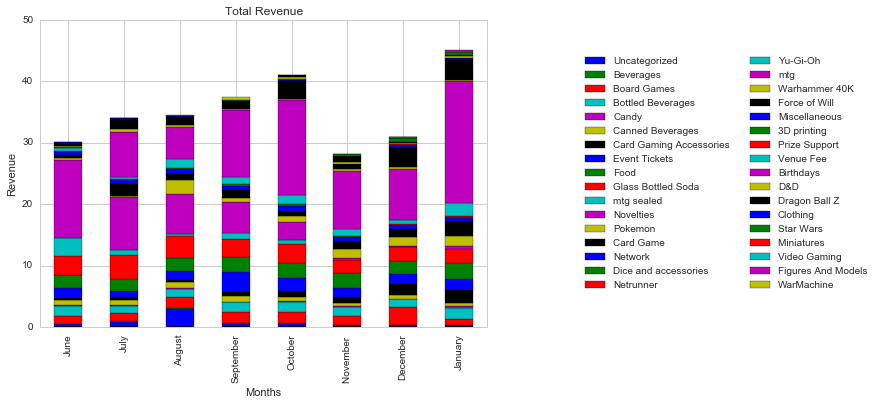
\includegraphics[width=.99\columnwidth]{TotalMonthlyRevenue}
\newline
There are some changes to weekly events that we believe should be made that would be helpful for The District Company.  Some weekly events seem to increase sales more than others, as shown in the tables below. Yu-Gi-Oh and Pokemon both have higher sales on the days that their events are held and on the days around the events. Tuesday�s events in particular should be changed.  Board Game sales do not increase at all on days with Board Game events, their sales are highest on Saturday, while there is a weekly Board Game night on Tuesdays. In fact, Tuesday does not have any category that has increased sales. This means the events on Tuesdays are probably not doing much to increase sales.
\newline
The District Company may want to get rid of the Wednesday Warhammer event, or market it differently.  The category for Warhammer does not always have an increase in sales when there is an event. There is a weekly event called Warhammer 40k Casual play that is on Mondays and Wednesdays. However, there is an increase in Warhammer sales on Mondays, but not on Wednesdays.  This means that in order for the Wednesday event to be as successful, The District Company may want to rethink some marketing strategies.
\newline
\vspace{10cm}
\begin{center}
\begin{center} District's Weekly Events \end{center}
\vspace{0.3cm}
\begin{tabular}{ m{1.9 cm} | m{1.4 cm} | m{1.9 cm} | m{1.7 cm} | m{1.2 cm} | m{1.4 cm} | m{1.2 cm}}
Monday & Tuesday & Wednesday & Thursday & Friday & Saturday & Sunday
\\
\hline
\hline
{Modern Monday}

& {Board Game Night }
& { Magic: The Gathering }
&{\color{red} Yu-Gi-Oh! Tournament }
& { \color{blue} Friday night Magic }
& { Super Smash Bros Wii U }
&{ Kids Board-Game Teach-\&-Play }
\\
\hline
{Star Wars X-Wing Miniatures Game }
& {EDH/ Commander meet up! }
& { \color{green} Warhammer 40k Casual Play }
&{ Board Game Night }
& { \color{blue} Booster Draft }
& { Force of Will Tournament }
&{ Dungeons and Dragons: Expeditions }
\\
\hline

{\color{green}Warhammer 40k Casual Play }
& {Game Designer Meet-up }
& { Star Wars X-Wing Miniatures Game }
&{ Throwback Thursday }
& { }
& { Magic the Gathering Chaos Draft }
&{\color{orange} Pokemon Trading Card Game League }
\\
\hline

\end{tabular}

\vspace{1.5 cm}
\end{center}



\vspace{10cm}

\begin{center}
\begin{center} Best Categories For The Days of The Week \end{center}
\vspace{0.3cm}
\begin{tabular}{ m{1.9 cm} | m{1.4 cm} | m{1.7 cm} | m{1.5 cm} | m{1.4 cm} | m{1.5 cm} | m{1.5 cm}}
Monday & Tuesday & Wednesday & Thursday & Friday & Saturday & Sunday
\\
\hline
\hline
{\color{orange} Pokemon}
& { }
& { }
&{ }
& { }
& {\color{orange} Pokemon }
&{\color{orange} Pokemon }
\\
\hline
{ }
& { }
& { }
&{ }
& { Network }
& { Network }
&{ Network }
\\
\hline

{ }
& { }
& { }
&{ }
& { Dice and accessories }
& {Dice and accessories }
&{ Dice and accessories }
\\
\hline

{ }
& { }
& { }
&{ \color{red} Yu-Gi-Oh }
& { \color{red} Yu-Gi-Oh }
& { \color{red} Yu-Gi-Oh }
&{ \color{red} Yu-Gi-Oh }
\\
\hline

{\color{green} Warhammer }
& { }
& { }
&{ }
& { }
& { }
&{ }
\\
\hline

{ }
& { }
& { Dragon Ball Z }
&{ }
& { Dragon Ball Z }
& { Dragon Ball Z }
&{ }
\\
\hline

{ }
& { }
& { }
&{ Video Gaming }
& { }
& { Video Gaming }
&{ Video Gaming }
\\
\hline

{ }
& { }
& { }
&{ }
& {\color{blue} Event Tickets }
& { }
&{ }
\\
\hline

{ }
& { }
& { }
&{ }
& { Card Games }
& { }
&{ }
\\
\hline

{ }
& { }
& { }
&{ }
& { D\&D }
& { }
&{ }
\\
\hline

{ }
& { }
& { }
&{ }
& { }
& { Beverages }
&{ Beverages }
\\
\hline

{ }
& { }
& { }
&{ }
& { }
& { Board Games }
&{ }
\\
\hline

{ }
& { }
& { }
&{ }
& { }
& { Force of Will }
&{ }
\\
\hline

\end{tabular}

\vspace{1.5 cm}
\end{center}

\newline
A big realization we came across that would help The District Company greatly is
their price of beverages, specifically Glass Bottled Beverages.  Using three different methods of analysis, it was revealed that the price of Glass Bottled Beverages should be increased.  By looking at all of the categories and comparing their total number of items sold and their total net sales, it was found that these types beverages had the highest number of sales, but the total net sales were among the lowest of the categories, as shown in Figure 2.  Therefore, in order to reach an equilibrium between all categories, the price should be raised.  This was the same result when looking at the relationship between each food/beverage category with the most successful gaming categories using multiple regression.  Glass Bottled Soda had some of the better correlations with each gaming category, meaning there is a demand for this product.  If the client were to raise the price, they would be able to make a little more profit considering there is a market for it.
\newline
The change with Glass Bottled Soda also came up when using simple linear regression to compare between the different types of beverages and food.  Out of the four categories of beverages, three of them show almost no correlation with food.  However, the Bottled Beverages category has a positive correlation with food sales. This means that when people buy food, they buy bottled beverages the most, but they do not buy as much of the other beverages with food. The District Company may want to use this information by encouraging customers to buy other beverages when they buy food.
\begin{figure}[b]
\begin{multicols}{2}

\begin{minipage}[t]{7.5cm}
  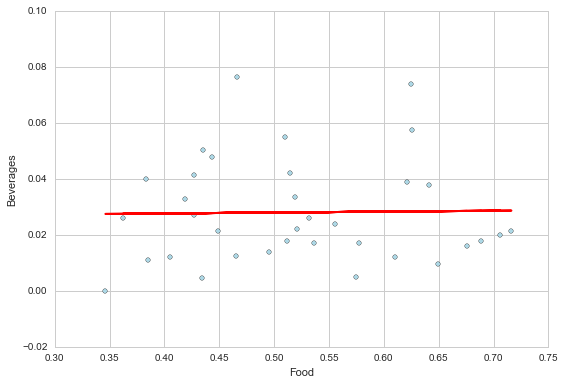
\includegraphics[width=.99\columnwidth]{Bev&Food}
  \begin{center}
  (a)
  \end{center}
  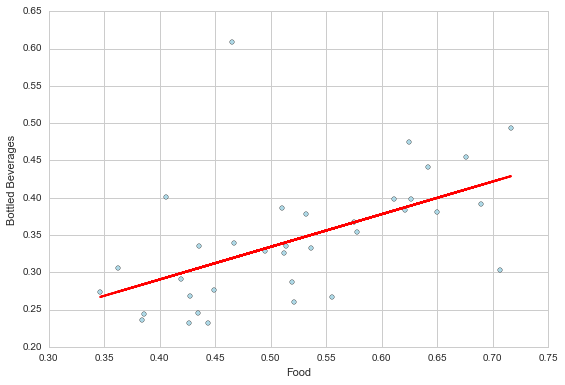
\includegraphics[width=.99\columnwidth]{Bottled&Food}
  \begin{center}
  (b)
  \end{center}
\end{minipage}

\columnbreak

\begin{minipage}[t]{7.5cm}
  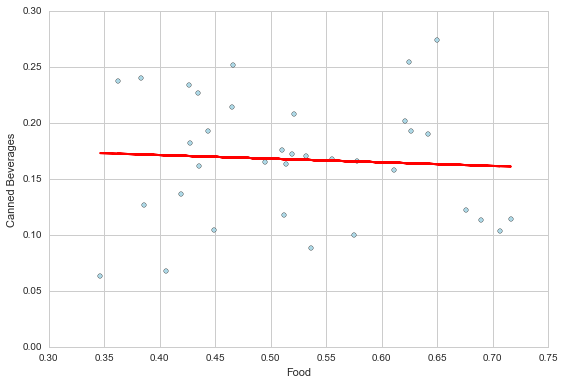
\includegraphics[width=.99\columnwidth]{Canned&Food}
  \begin{center}
  (d)
  \end{center}
  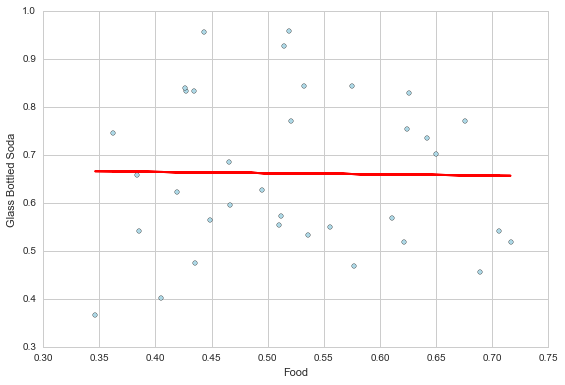
\includegraphics[width=.99\columnwidth]{Glass&Food}
  \begin{center}
  (e)
  \end{center}
\end{minipage}
\end{multicols}

\caption{Here are some graphs.}\label{fig:Graphs}
\end{figure} 
\newline
The fact that Bottled Beverages and food have a higher correlation becomes an interesting point when being compared with D\&D through multiple regression.  When looked at more closely, it was found that Bottled Beverages and food have a negative correlation with D\&D sales.  This means that people who are playing D\&D are not buying Bottled Beverages or food.  The District Company may want to take this information and market these items better during the D\&D events.
\newline
\begin{center}
\begin{center}Before D\&D By Days\end{center}
\vspace{0.3cm}
\begin{tabular}{ c || c | c | c | c | c |}
$x/y$ down & MTG & D\&D & Novelties & Event Tickets & Board
Games\\
\hline
\hline
Beverages & {\color{blue}0.001} & {\color{blue}0.010} &
{\color{blue}0.005} & {\color{blue}-0.004} & {\color{blue}-0.007} \\
\hline
Bottled Beverages & {\color{blue}0.020} & {\color{blue}-0.041} &
{\color{blue}0.030} & {\color{blue}0.052} & {\color{blue}0.088} \\
\hline
Food & {\color{blue}0.026} & {\color{orange}0.107} &
{\color{blue}0.033} & {\color{blue}0.085} & {\color{orange}0.104} \\
\hline
Glass Bottle Beverages & {\color{blue}0.032} & {\color{blue}0.089} &
{\color{orange}0.137} & {\color{blue}0.015} & {\color{orange}0.185} \\
\hline
Canned Beverages & {\color{blue}0.003} & {\color{blue}0.023} &
{\color{blue}0.026} & {\color{blue}0.026} & {\color{blue}0.015} \\
\hline
Candy & {\color{blue}0.003} & {\color{blue}0.009} &
{\color{blue}-0.003} & {\color{blue}0.0001} & {\color{blue}0.002} \\
\hline
\end{tabular}
\begin{center}
% \begin{tablenotes}
{{\color{green} greater than 1.0},
{\color{magenta}0.51 to 0.99}, {\color{orange}0.1 to 0.5},
{\color{blue} less than 0.1}}
% \end{tablenotes}
\end{center}

\end{center}

\newline

\begin{center}
\begin{center}After D\&D By Weeks\end{center}
\vspace{0.3cm}
\begin{tabular}{ c || c | c | c | c | c |}
$x/y$ down & MTG Combined & D\&D & Novelties & Event Tickets & Board
Games\\
\hline
\hline
Beverages & {\color{blue}-0.004} & {\color{blue}0.017} &
{\color{blue}0.024} & {\color{blue}-0.014} & {\color{blue}-0.024} \\
\hline
Bottled Beverages & {\color{blue}0.014} & {\color{orange}-0.236} &
{\color{blue}0.085} & {\color{blue}-0.012} & {\color{blue}0.034} \\
\hline
Food & {\color{blue}0.031} & {\color{orange}-0.230} &
{\color{blue}0.037} & {\color{blue}0.094} & {\color{blue}0.092} \\
\hline
Glass Bottle Beverages & {\color{blue}0.023} & {\color{orange}0.261} &
{\color{orange}0.188} & {\color{blue}0.023} & {\color{blue}0.084} \\
\hline
Canned Beverages & {\color{blue}-0.006} & {\color{blue}0.023} &
{\color{blue}0.023} & {\color{blue}0.084} & {\color{blue}-0.024} \\
\hline
Candy & {\color{blue}0.003} & {\color{blue}0.070} &
{\color{blue}-0.025} & {\color{blue}0.004} & {\color{blue}-0.017} \\
\hline
\end{tabular}
\begin{center}
%\begin{tablenotes}
{{\color{green} greater than 1.0},
{\color{magenta}0.51 to 0.99}, {\color{orange}0.1 to 0.5},
{\color{blue} less than 0.1}}
%\end{tablenotes}



\end{center}
\end{center}

\newline
One important data analytic technique we were able to employ was the ability to decrease the scope, or point of view.  This is best presented when we find that a category is either doing really well in one aspect but poorly in another.  For example, if Bottled Beverages are doing well in correlation with food, there is good reason to dig deeper into the data analysis and see why this is happening.  This correlation may be because of many different things but one main reason could be because one bottled beverage is doing well compared to the rest.  If this is the case, then there is strong evidence that we should increase prices on that beverage to increase profit.





\subsection*{\hspace{-.5cm} Problems to consider.}\label{tech}
Most of our results are fairly weak because we might not have good enough relationships to make decisions. There is a good chance that we will not get our surveys back before the end of the semester. This is a big loss in data because we could have gotten insight on customers� wants and needs. There was a few concerns with the data too. Some categories overlap with each other, so they are not independent. The definition of the categories seem to be changing. We were told that the D\&D category did not start until three months into the data we were given. This results in three months of zero entries for this category and may skew our results. Both the overlap and the addition/removal of categories is a concern because there may be more of these situations than we are aware.
\subsection*{\hspace{-.5cm} Conclusion.}\label{tech}
Through this project we learned about statistical analysis using linear regression, classifiers, and Python. We used that to help The District Company make decisions about marketing. We were able to come up with some results that may help them. There were correlations with some of the categories and there were events that were not helping improve sales. Even with some of the problems we had, we are confident with the results we were able to obtain.




\begin{figure}[c]
\begin{multicols}{2}

\begin{minipage}[t]{7.5cm}
  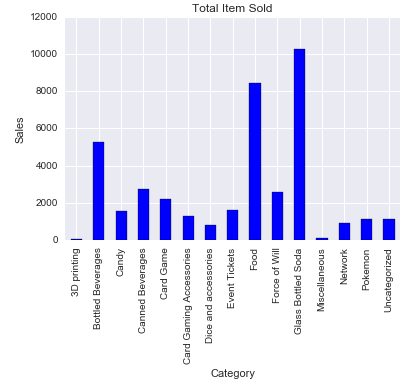
\includegraphics[width=.99\columnwidth]{TotalItemsSold}
  \begin{center}
  (a)
  \end{center}
\end{minipage}

\columnbreak

\begin{minipage}[t]{7.5cm}
  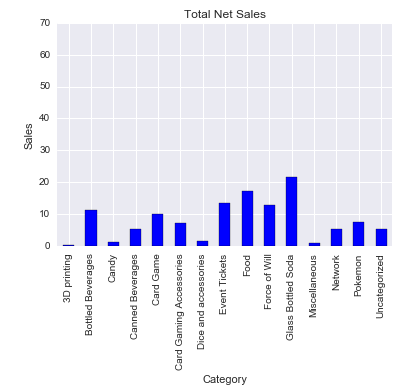
\includegraphics[width=.99\columnwidth]{TotalNetSales}
  \begin{center}
  (b)
  \end{center}

\end{minipage}
\end{multicols}
\caption{Total Items Sold and Total Net Sales.}\label{fig:Graphs}
\end{figure}













\end{document}

